\section{Bestimmtes und unbestimmtes Integral}\label{sec:integral}

Ein Integral $\int_a^b f(x) \d x$ kann man sich als die Fläche unter einem Kurvenstück vorstellen.
\begin{center}
    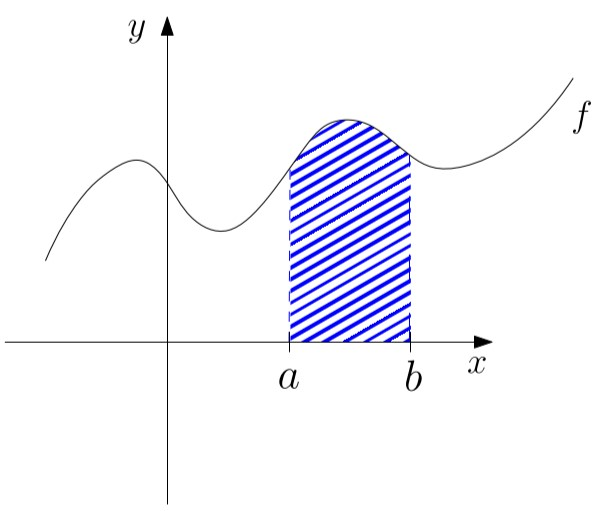
\includegraphics[scale=0.3]{integral}
\end{center}

\subsection{Der Hauptsatz der Differential- und Integralrechnung}\label{subsec:hauptsatz-integralrechnung}

\begin{definition}{Stammfunktionen}
    Gegeben sind ein Intervall $I \subset \R$ und eine Funktion $f : I \rightarrow \R$.
    Eine \emph{Stammfunktion} von $f$ ist eine Funktion $F$, für die gilt: \[F'(x) = f(x)\] für alle $x \in I$.
    D.h.\ wenn man die Stammfunktion ableitet, ergibt sich wieder die Funktion $f$.
\end{definition}

\textbf{Beispiel:} Die Funktion $f(x) = 2x + 1$ hat die Stammfunktionen $F_1(x) = x^2 + x$ und $F_2(x) = x^2 + x + 42$.

Der untenstehende Satz ist Teil vom sogenannten \textbf{Hauptsatz der Differential- und Integralrechnung}.

\begin{definition}{Satz}
    Gegeben ist eine Funktion $f$, die auf einem Intervall $I$ stetig ist, und eine beliebige Stammfunktion $F$ von $f$.
    Dann gilt für alle $a,b \in I$: \[\int_a^b f(x) \d x = F(b) - F(a).\]
\end{definition}

\textbf{Bemerkung:} Das \emph{unbestimmte} Integral $\int f(x) \d x$ bezeichnet eine ``allgemeine'' Stammfunktion der Funktion $f(x)$: \[\int f(x) \d x = F(x) + c\]
Dabei lässt man offen, für welche reelle Zahl die sogenannte \emph{Integrationskonstante} $c$ steht.

\textbf{Achtung:} $\int_a^b f(x) \d x$ ist eine Zahl, $\int f(x) \d x$ ist eine Funktion!

\begin{definition}{Integrationsregeln}
    Gegeben sind zwei Funktion $f$ und $g$ mit Stammfunktionen $F$ bzw. $G$ sowie eine Konstante $c$.
    Dann gilt:
    \begin{enumerate}
        \item $c \cdot F(x)$ ist eine Stammfunktion von $c \cdot f(x)$
        \item $F(x) + G(x)$ ist eine Stammfunktion von $f(x) + g(x)$
    \end{enumerate}
\end{definition}
\begin{definition}{}
    Zusammen mit dem Hauptsatz der Integralrechnung lässt sich daraus folgendes ableiten:
    \begin{enumerate}
        \item $\int_a^b c \cdot f(x) \d x = c \cdot \int_a^b f(x) \d x$
        \item $\int_a^b (f(x) + g(x)) \d x = \int_a^b f(x) \d x + \int_a^b g(x) \d x$
    \end{enumerate}
\end{definition}

\newpage

\textbf{Bemerkung:} Es gibt keine entsprechenden Formeln für Produkte und Quotienten, im Allgemeinen gilt aber: \[\int_a^b (f(x) \cdot g(x)) \d x \neq \left(\int_a^b f(x) \d x\right) \cdot \left(\int_a^b g(x) \d x\right)\] und \[\int_a^b \frac{f(x)}{g(x)} \d x \neq \frac{\int_a^b f(x) \d x}{\int_a^b g(x) \d x}\]

\subsection{Integration von Polynomfunktionen}\label{subsec:integration-polynomfunktionen}

Dank dem Hauptsatz der Differential- und Integralrechnung lässt sich das Integrieren auf das Finden von Stammfunktionen zurückführen.

\textbf{Beispiel 1:} Stammfunktion von $f(x) = c$.

\RIGHTarrow Gesucht ist eine Funktion $F(x)$, sodass $F'(x) = c$.
Die Lösung ist $F(x) = c \cdot x$.

\textbf{Beispiel 2:} Stammfunktion von $f(x) = x^n$ mit $n \in R, n \neq -1$

\RIGHTarrow Gesucht ist eine Funktion $F(x)$, sodass $F'(x) = x^n$.
Die Lösung ist $F(x) = \frac{1}{n + 1} \cdot x^{n + 1}$.

Man kann diese Beispiele verallgemeinern:
\begin{definition}{Satz}
    Für alle $n \in \Z$ mit $n \neq -1$ gilt: \[F(X) = \frac{1}{n + 1} \cdot x^{n + 1}\] ist eine Stammfunktion von $f(x) = x^n$.
\end{definition}

\subsection{Ableitungen und Integrale einiger ausgewählter Funktionen}\label{subsec:ableitungen-und-integrale-funktionen}

\subsubsection*{Potenz- und Logarithmusfunktionen}

\begin{itemize}
    \item $\int a^x \d x = \frac{a^x}{\ln(a)} + C$
    \item $\int \ln(x) \d x = x \cdot \ln(x) - x + C$
    \item $\int \log_a(x) \d x = \frac{1}{\ln(a)} \cdot (x \cdot \ln(x) - x) + C$
\end{itemize}

\subsubsection{Trigonometrische Funktionen}

\begin{itemize}
    \item $\int \sin(x) \d x = -\cos(x) + C$
    \item $\int \cos(x) \d x = \sin(x) + C$
    \item $\int \tan(x) \d x = -\ln |\cos(x)| + C$
    \item $(\tan(x))' = 1 + \tan^2(x) = \frac{1}{\cos^2(x)} \quad$ resp. $\int (1 + \tan^2(x)) \d x = \int \frac{1}{\cos^2(x)} \d x = \tan(x) + C$
    \item $(\arcsin(x))' = (1 - x^2)^{-1/2} \quad$ resp. $\int (1 - x^2)^{-1/2} \d x = \arcsin(x) + C$
    \item $(\arccos(x))' = -(1 - x^2)^{-1/2} \quad$ resp. $\int -(1 - x^2)^{-1/2} \d x = \arccos(x) + C$
    \item $(\arctan(x))' = (1 + x^2)^{-1} \quad$ resp. $\int (1 + x^2)^{-1} \d x = \arctan(x) + C$
\end{itemize}